\usetikzlibrary{matrix}


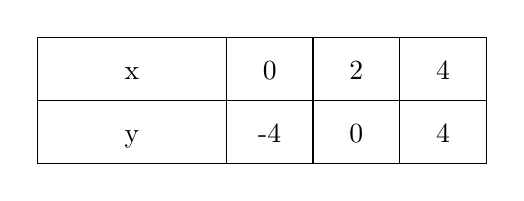
\begin{tikzpicture}

\matrix (table) [
  matrix of nodes,
  nodes={draw, minimum height=0.8cm, text depth=0.25ex, text height=2ex, anchor=center},
  column 1/.style={nodes={minimum width=2.4cm}},
  column 2/.style={nodes={minimum width=1.1cm}},
  column 3/.style={nodes={minimum width=1.1cm}},
  column 4/.style={nodes={minimum width=1.1cm}},
  column 5/.style={nodes={minimum width=1.1cm}},
  column 6/.style={nodes={minimum width=1.1cm}},
  column 7/.style={nodes={minimum width=1.1cm}},
  row sep=-\pgflinewidth,
  column sep=-\pgflinewidth
]
{
  {x} & 0 & 2 & 4 \\
  {y} & -4 & 0 & 4 \\
};

\end{tikzpicture}